\chapter{Маршрут проектирования микросхем}\label{appendix:ic-route}

\dictum[]{\todo dictum.}

\section{Введение}
    
В некоторый момент проектирование нового устройства переходит от симуляций различной степени точности, циклов уточнения спецификаций и создания синтезируемого описания на соответствующих языках к заключительному этапу: разработка описания микросхемы, пригодного для отправки на фабрику, на которой будет изготовляться продукция.

В данной главе описывается т.н. маршрут проектирования, т.е. отдельные этапы структурированного процесса создания работоспособного и отлаженного продукта.

Проектирование интегральных схем --- процесс, зачастую требующий возвращения к ранее пройденной фазе проектирования под влиянием данных, полученных на поздних этапах, для уточнения или даже полного пересмотра результатов его работы. Ниже приведены краткая информация обо всех типичных этапах в порядке их прохождения без учёта корректирующих возвратов. Детальное описание каждой из них выходят за рамки данной книги. Читателю, желающему более подробно разобраться с данным вопросом, рекомендуется обратиться к обширной специализированной литературе~\cite{books/daglib/0027783, dicd}.

\section{Логическое проектирование}

Логическое проектирование (\abbr logic design) --- начальная стадия, базирующаяся на основе технического задания и используемых средств автоматизации (например, программного обеспечения).

Применяемые на данном этапе абстракции:
\begin{itemize*}
    \item модули памяти представлены в виде <<чёрных ящиков>> библиотечных макро--модулей;
    \item уровень представления логических элементов ограничен регистрами и передачей данных между ними --- RTL (\abbr register transfer level).
\end{itemize*}

Часто работа ведётся в специализированном графическом редакторе, непосредственно отображающем иерархические блоки схемы.

\section{Логический синтез}\label{logicsynthesis}

На данной фазе в рассмотрение вводится ряд физических параметров проектируемой системы, таких как ограничения по мощности отдельных компонентов и всей схемы, ограничения и особенности выбранной технологии. Однако пока не учитываются временн\textit{ы}е характеристики используемых модулей. Результатом этого этапа является получение описания устройства в формате \textit{списка связей} (\abbr netlist).

\section{Анализ задержек}

На данном этапе происходит введение в рассмотрение учёта длительности задержек отдельных элементов. В свою очередь это ограничивает допустимые варианты расположения и соединения узлов на кристалле. Поэтому результаты фазы оказывают влияние на все последующие моменты проектирования.

\section{Проектирование для проведения первого тестирования}

Целью данного этапа является тестирование описания на соответствие полученных промежуточных результатов исходному заданию. Это позволит обнаружить ошибки, которые в дальнейшем могли бы существенно повлиять на результат всего проектирования. Используется netlist, полученный при логическом синтезе. Кроме того, происходит раскрытие некоторых деталей внутреннего устройства некоторых блоков, до этого считавшихся неделимыми.

\section{Планирование размещения блоков}

Первоначальное грубое размещение блоков элементов на доступной площади кристалла (\abbr floorplanning). При этом учитываются геометрические ограничения на размер, положение и взаимное расположение отдельных блоков. Алгоритмическая сложность нахождения оптимального решения для задачи размещения в общем случае является значительной. Как и многие другие проблемы, возникающие на разных этапах проектирования, она является NP-сложной.

Кроме того, в качестве результата планирования происходит получение уточнённых данных о задержках передачи сигналов между модулями. 

% \section{Первичное размещение}\label{floorplanning}

% Уточнение положения отдельных компонент на плате с учётом ограничений, накладываемых на чип. Получение уточнённых данных о  задержках передачи сигналов между модулями. 

% \section{Проектирование для проведения второго тестирования (Design for test)}\label{test2}
% 
% \todo ??

\section{Построение дерева задержек}

В современной интегральной схеме, работающей на частоте, превышающей 1ГГц, подведение единого сигнала от тактового генератора ко всем её элементам с сохранением правильной задержки и формы сигнала не представляется возможным: для разных частей длина пути до источника сигнала различна. Кроме того, фактор нагруженности (сила тока) подобной шины был бы в таком сучае огромен. Поэтому в использование вводится понятие домена синхронизации (\abbr clock domain). В каждом домене изменения тактового сигнала синхронно подаются на все элементы. Дополнительно, каждый домен имеет фиксированную задержку относительно других, что упрощает синхронизацию сигналов, пересекающих их границы.

В результате этого этапа проектирования создаётся иерархическая структура --- дерево доменов, --- размещённая на плоскости кристалла. На рис.~\ref{fig:htree} приведена фрактальная структура, т.н. \textit{H-дерево}. Геометрические свойства отдельных его ветвей делают его удобным для построения деревьев задержек.

% H-tree fractal for TiKZ/PGF.
% Taken from http://pbelmans.wordpress.com/2010/12/27/an-h-tree-in-tikz/
% Author: Pieter Belmans
\pgfdeclaredecoration{H-tree}{init}
{
  \state{init}[width=\pgfdecoratedinputsegmentremainingdistance]
  {
    \pgfpathmoveto{\pgfpoint{0pt}{0.35355\pgfdecoratedinputsegmentremainingdistance}}
    \pgfpathlineto{\pgfpoint{0pt}{-0.35355\pgfdecoratedinputsegmentremainingdistance}}
    \pgfpathmoveto{\pgfpoint{0pt}{0pt}}
    \pgfpathlineto{\pgfpoint{\pgfdecoratedinputsegmentremainingdistance}{0pt}}
    \pgfpathmoveto{\pgfpoint{\pgfdecoratedinputsegmentremainingdistance}{0.35355\pgfdecoratedinputsegmentremainingdistance}}
    \pgfpathlineto{\pgfpoint{\pgfdecoratedinputsegmentremainingdistance}{-0.35355\pgfdecoratedinputsegmentremainingdistance}}
    \pgfpathmoveto{\pgfpoint{\pgfdecoratedinputsegmentremainingdistance}{0pt}}
  }
}
\begin{figure}
\centering
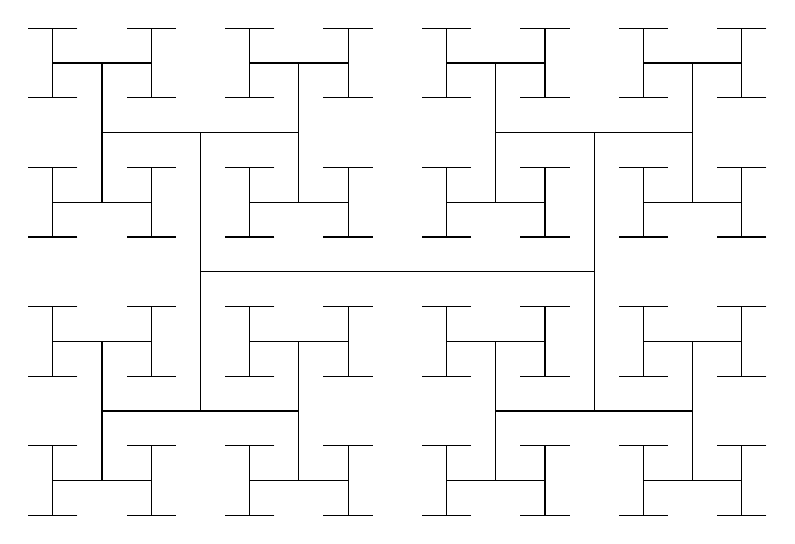
\begin{tikzpicture}[decoration=H-tree]
  \draw decorate{decorate{decorate{decorate{decorate{decorate{ (0,0) -- (5,0) }}}}}};
\end{tikzpicture}
    \caption{H-дерево, первые 6 уровней}
    \label{fig:htree}
\end{figure}

\section{Трассировка}\label{trace}

Трассировка (\abbr routing) --- проложение путей между контактными выводами отдельных блоков, размещённых на чипе на этапе планирования размещения. Решаемые при этом задачи:
\begin{itemize*}
    \item соединить все точки, связи между которыми существют в netlist'е;
    \item не соединять точки, между которыми не должно быть связей;
    \item выдержать требования на задержки, допустимую плотность проложения связей, минимизировать перекрёстные помехи (\abbr crosstalk);
    \item выполнить прочие установленные для выбранного технического процесса правила и ограничения, диктуемые его физическими особенностями.
\end{itemize*}

\section{Логическая верификация}\label{logicverif}

На данной фазе проверяется, что логика работы создаваемой цифровой схемы сохранена, и в неё не было внесено ошибок на предыдущих этапах. Для этого необходимо удостовериться, что сигналы, поданные на вход схемы, вызвают ожидаемые изменения значений на её выходах.

\section{Формальная верификация}

Дополнительная стадия проверки корректности соответствия текущего описания интегральной схемы спецификациям, полученным в начале маршрута.

% Проведение сравнения netlist'ов с различных этапов для выявления ошибок, внесённых на поздних стадиях.

\section{Симуляция на тестовых векторах}

Используются результаты работы этапа \ref{logicverif} для получения тестовых векторов --- значений на входе схемы, для которых будут сличаться значения выходных сигналов. Проводится симуляция схемы. При этом модель формируется на основе описаний, полученных на стадии трассировки~\ref{trace}.

\section{Физическая верификация}

Проверка физических параметров проектируемого кристалла (размеры, плотность расположения соединений и элементов и т.п.) на пригодность для производства на конкретной фабрике.

\subsection{Верификация путей трассировки}

Дполнительная проверка на соответствие полученной схемы расположения и связей между элементами предполагаемым размерам кристалла.

\subsection{Проверка компоновочной схемы на соответствие принципиальной схеме (Layout vs Schematic tests)}

\todo{Написать}

\section{Отправка на фабрику}
    
Чертежи отправляются на фабрику-изготовитель кристаллов. На данном этапе внесение изменений в дизайн становится практически невозможным.
    
\iftoggle{webpaper}{
    \printbibliography[title={Литература}]
}{}

